\chapter{\leavevmode \newline Literature Review}
\label{chap:Literature Review}

Autonomous navigation in unknown, unstructured environments poses a complex challenge, especially when sensing is limited to proprioceptive input and the terrain is composed of granular material that can deform unexpectedly underfoot. In such settings, traditional visual mapping approaches often fail, and the robot must rely entirely on local interaction to evaluate risk and plan its movement. Addressing this problem requires methods that can reason under uncertainty, ensure safety without full knowledge of the environment, and adapt motion in real time based on new evidence.

This chapter reviews two key areas of related work that inform the development of \algoname. The first involves Bayesian optimization and Gaussian Process-based modeling to handle uncertainty and guide safe exploration. The second includes reactive control strategies, particularly those based on Voronoi and power diagram constructions, which enable real-time, geometry-aware navigation in partially known or dynamic spaces. These approaches together form the conceptual backbone of \algoname, though the system departs from prior work by operating entirely on proprioceptive sensing in visually degraded environments.

\section{Bayesian Optimization and Gaussian Processes in Navigation}

Bayesian optimization techniques have become powerful tools for exploration under uncertainty. They use statistical models—typically Gaussian Processes (GPs)—to approximate unknown functions and select informative or optimal sampling points. In robotic navigation, this framework allows the robot to learn about the environment while avoiding unsafe terrain.

\textcite{muenprasitivej2024bipedalsafenavigationuncertain} employ GPs to model terrain elevation and uncertainty for bipedal robots. Their method integrates footstep planning with information gain objectives, enabling safe exploration even in unstable regions. This work highlights how GP-based models can unify terrain understanding with locomotion constraints, but it assumes exteroceptive input such as elevation maps.

\textcite{uttsha2024gaussianprocessdistancefields} generalize this idea by creating GP-based distance fields from 3D point clouds. Their system constructs smooth elevation and obstacle maps that support planning for legged and wheeled robots. The result is a flexible, continuous representation of traversability that allows robust trajectory optimization in uneven terrain. This framework, however, requires point cloud sensing, which may not be feasible in degraded visual conditions.

\textcite{leininger2024gaussianprocessbasedtraversabilityanalysis} extend these ideas using Sparse GPs to build terrain cost maps and steer an RRT* planner. Their approach selects subgoals along the frontier to guide the robot while minimizing exposure to uncertain regions. However, it relies on global terrain observations and sampling-based planning, which can be computationally expensive and poorly suited to real-time reactivity.

All of these methods demonstrate the power of GPs for terrain-aware planning, but most require exteroceptive sensors and rely on offline or batch planning. In contrast, \algoname{} uses proprioceptive data only, incrementally building a risk model in real time and making decisions at the resolution of physical contact.

\subsection{Gaussian Process Upper Confidence Bound (GP-UCB)}

The GP-UCB algorithm provides a principled approach for choosing sampling points when both uncertainty and performance must be considered. It selects the next query location \( x \) by maximizing:
\[
a_{\text{UCB}}(x) = \mu_{n-1}(x) + \beta\, \sigma_{n-1}(x)
\]
where \( \mu \) and \( \sigma \) represent the GP’s posterior mean and uncertainty, and \( \beta \) scales the confidence margin. This algorithm efficiently balances exploration (uncertain points) and exploitation (high-performing predictions).

In \algoname{}, a similar confidence-aware sampling strategy is used, but applied spatially to terrain traversal. Instead of seeking optima, the goal is to incrementally grow a certified safe set based on proprioceptive risk estimates.

\subsection{Safe Bayesian Optimization (SafeOpt)}

SafeOpt builds on GP-UCB by enforcing that each function evaluation satisfy a minimum safety constraint:
\[
f(x) \geq h
\]
with high probability. It maintains and expands a set of safe decisions while seeking high performance, avoiding evaluations in dangerous regions.

\algoname{} adapts this paradigm to navigation by only sampling locations where terrain risk is predicted to fall below a safety threshold. While not a direct implementation of SafeOpt, the core idea of conservative, uncertainty-aware expansion is central to its planning mechanism.

\section{Reactive Navigation Using Voronoi-Based Methods}

Whereas GP-based methods focus on estimating terrain and selecting strategic waypoints, reactive navigation methods address a complementary need: executing safe, collision-avoiding motion in real time as new obstacles are discovered.

\subsection{Navigation in Convex Worlds}

\textcite{arslan2016exactrobotnavigation} propose a method that uses power diagrams to define convex, obstacle-free regions around the robot. Within these regions, a local optimization strategy guides the robot toward its goal. The method guarantees convergence from almost all starting positions and is highly efficient due to its geometric construction.

\textcite{arslan2016sensorbasedreactive} extend this framework to unknown environments by using local sensing to infer separating hyperplanes and construct reactive control fields. Their system allows real-time motion in cluttered spaces using only local information.

These methods inspire the reactive control layer in \algoname. By constructing convex approximations of safe space based on proprioceptive estimates rather than direct obstacle detection, \algoname{} achieves comparable responsiveness using internal sensing alone.

\subsection{Navigation in Concave and Partially Known Worlds}

\textcite{Vasilopoulos_RAL_2020} combine semantic SLAM with reactive control to navigate through cluttered, dynamic environments. Their robot adjusts its plan in real time based on object detection and scene understanding, enabling smooth motion even in rapidly changing spaces.

This work is extended in \textcite{vasilopoulos2021reactivenavigationpartiallyfamiliar}, where robots use semantic labels to decide whether to trust a prior map or act reactively. This hybrid strategy improves efficiency by leveraging prior structure while maintaining responsiveness to new hazards.

In contrast, \algoname{} constructs hazard boundaries from terrain risk estimates, not visual or semantic input. The use of proprioceptive sensing makes it viable in visually degraded environments such as planetary surfaces, where dust, shadowing, or lack of light renders cameras ineffective.

\begin{figure}[h]
\centering
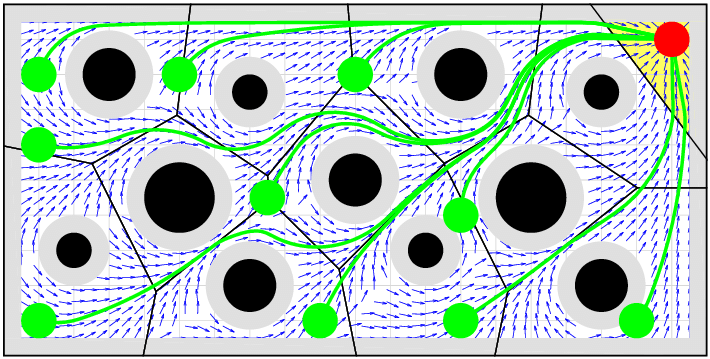
\includegraphics[width=0.7\linewidth]{figures/Exact-robot-navigation-using-power-diagrams-generated-by-disks-representing-obstacles.png}
\caption{Exact robot navigation using power diagrams, generated by disks representing obstacles (black) and the robot (red at the goal). The power cell (yellow) associated with the robot defines its obstacle free convex local neighborhood, and the continuous feedback motion towards the metric projection of a given desired goal (red) onto this convex set asymptotically steers almost all robot configurations (green) to the goal without collisions along the way. The grey regions represent the augmented workspace boundary and obstacles, and the arrows show the direction of the resulting vector field. \cite{arslan2016exactrobotnavigation}}
\label{fig:disks}
\end{figure}

\subsection{Other Voronoi-Based Techniques}

\textcite{garrido2015mobilerobotpathplanning} use Voronoi diagrams with the Fast Marching Method to compute paths with maximal clearance in real time. Their technique supports continuous updates as new obstacles are sensed, reinforcing the need for responsiveness in dynamic settings.

\algoname{} shares this emphasis on responsiveness, but relies on inferred terrain risk to shape its navigation domain, rather than explicit obstacle maps. The underlying philosophy—a robot should move cautiously through space while dynamically updating its understanding of nearby hazards—is closely aligned.

\section{Summary and Motivation for This Work}

Prior work in terrain-aware navigation has demonstrated the power of both probabilistic modeling and reactive control. Gaussian Processes enable safe and data-efficient exploration by modeling uncertainty, while Voronoi-based planners enable fast, obstacle-avoiding motion with minimal computation. However, these approaches have typically been applied in isolation, or require vision or global maps to function effectively.

\algoname{} integrates the most compelling aspects of these two paradigms: it uses confidence-guided expansion of safe terrain based on proprioceptive input, and it executes motion in real time using a reactive controller adapted from power diagram-based methods. This combination enables the robot to safely explore deformable granular terrain with no visual information, no global map, and no need for complete re-planning in response to environmental change.

In doing so, this work contributes a unified navigation architecture that is both safe and adaptive, capable of expanding its operational zone and navigating within it using only what the robot feels through its limbs.
